\documentclass{article}
\usepackage{graphicx} 
\usepackage{hyperref}

\title{Advanced programming for HPC}
\author{Son Dang Thai}
\date{September 2025}

\begin{document}

\maketitle

\section{Device name}
After importing cuda from numba, using cuda.select\_device() with id 0, the device name was shown as "NVIDIA GeForce GTX 1650".

\section{Core information}
The number of multiprocessor could be easily retrieved using MULTIPROCESSOR\_COUNT which was 14.
\\For the number of cores, it was not displayed directly. This was computed by multiplying the number of multiprocessors and with the number of core on each multiprocessor. Based on \href{https://stackoverflow.com/questions/63823395/how-can-i-get-the-number-of-cuda-cores-in-my-gpu-using-python-and-numba}{this answer}, the latter is 64 according to my local device compute capability. Therefore, the total number of cores was 14*64=896.

\section{Memory information}
The free and total GPU memory were retrieved by cuda.current\_context().get\_memory\_info():
\begin{itemize}
    \item Free memory: 3311 MB
    \item Total memory: 4096 MB
\end{itemize}

\section{Overall result}
\begin{figure}
    \centering
    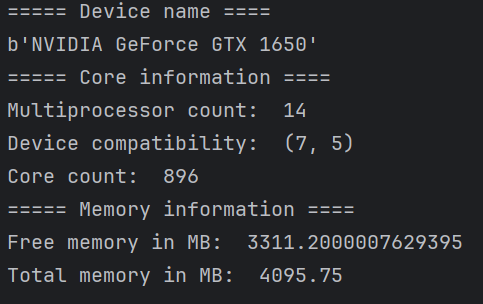
\includegraphics[width=1\linewidth]{Overall result.png}
    \caption{Overall result}
    \label{fig:placeholder}
\end{figure}

\end{document}
